\documentclass{beamer}
\usepackage{caption}
\captionsetup[figure]{font=scriptsize,labelfont=scriptsize}

% Choose your theme
\usetheme{Madrid}

% Title page information
\title{Probabilistic Modelling}
\author{Claire Zhang, Mikail Khona}
\date{\today}

\begin{document}

% Title slide
\begin{frame}
  \titlepage
\end{frame}

% Table of Contents
% \begin{frame}
%   \frametitle{Outline}
%   \tableofcontents
% \end{frame}

% Section 1
\section{Problem Setup}
\begin{frame}
    \frametitle{Problem}
    \begin{center}
        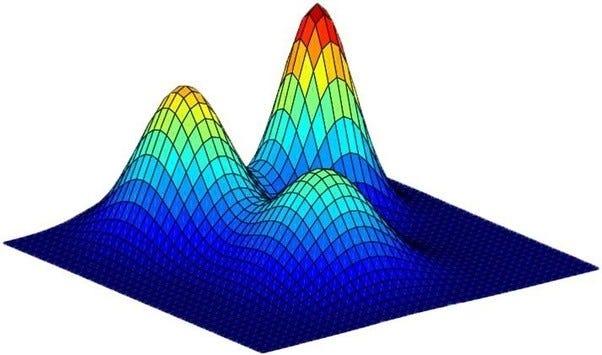
\includegraphics[width=0.5\textwidth]{images/gmix.jpg}
    \end{center}
    \begin{itemize}
    \item Given: $x_1, \ldots, x_N \sim p(x)$.
    \item Goal: Generate new samples according to $p(x)$.
    \item Uses:
        \begin{itemize}
            \item Generative modelling
            \item Unsupervised learning
            \item Data augmentation
        \end{itemize}
    \end{itemize}
\end{frame}

% Section 2
\section{Variational Inference}

\begin{frame}
\frametitle{Casual Model}
View the $X$ as the effect of a cause $Z$. Assume the data is generated as follows:

    \begin{itemize}
    \item $z \sim p(z)$
    \item $x \sim p(x|z)$
    \end{itemize}
    \[p_X(x) = \int p_Z(z) p_{X | Z}(x|z) dz\]
    We approximate $p(z)$ and $p(x|z)$ with parametric $p_{\theta}(z)$ and $p_{\theta}(x|z)$.

    \begin{block}{Goal}
        Find $\theta$ such that $p(x) \approx p_{\theta}(x)$.
    \end{block}
\end{frame}

\begin{frame}
    \frametitle{Variational Inference Goal}

    \begin{block}{Goal}
    Find $\theta$ that minimizes 
    \[D_{KL}(p || p_\theta) = \int  p(x) \log \frac{p(x)}{p_{\theta}(x)} dx\]
    \end{block}
    % \begin{align*}
    % \theta^* &= \arg \min_\theta D_{KL}(p_X || p_{X; \theta}) \\
    % &= \arg \min_\theta \int p_X(x) \log \frac{p_X(x)}{p_{X; \theta}(x)} dx \\
    % &= \arg \max_\theta \int  p_X(x) \log p_{X; \theta}(x) dx
    % \end{align*}
    ie. maximizes the average log-likelihood of data (EV of):
    \begin{align*}
        \log p_{\theta}(x) &= \log \int p_{\theta}(x, z) dz \\
        &= \log \int \frac{p_{\theta}(x, z)}{q_{\phi
        }(z|x)} q_{\phi}(z|x) dz \\
        &\geq \int q_\phi(z|x) \log \frac{p_{\theta}(x, z)}{q_\phi(z|x)} dz \\
        &= \mathbb{E}_{q_\phi(z|x)} \left[ \log \frac{p_\theta(z) p_{\theta}(x|z)}{q_\phi(z|x)} \right] \\
    \end{align*}
\end{frame}

\begin{frame}
    \frametitle{Evidence Lower Bound}
    \begin{align*}
        \mathcal{L}(\theta, \phi; x) &:= \mathbb{E}_{q_\phi(z|x)} \left[ \log \frac{p_\theta(z) p_{\theta}(x|z)}{q_\phi(z|x)} \right] \\
        &= \mathbb{E}_{q_\phi(z|x)} \left[ \log p_\theta(x|z) \right] - D_{KL}(q_\phi(z|x) || p_\theta(z)) \\
        &= \mathbb{E}_{p_\theta(\epsilon)} \left[ \log p_\theta(x|\mathbf{\phi}, \mathbf{\epsilon)} \right] - D_{KL}(q_\phi(z|x) || p_\theta(z)) 
    \end{align*}
    if we \textbf{reparameterize} $z = g_\phi(x, \mathbf{\epsilon})$, where $\epsilon \sim p_\theta(\epsilon)$.
    
    If $g_\phi$ is differentiable wrt. $\phi$, $\mathcal{L}(\theta, \phi; x)$ can be maximized with gradient descent.
\end{frame}

\begin{frame}
    \frametitle{Sampling}
    We sample $\tilde{x} \sim p_\theta(x)$ using $p_\theta(z)$ and $p_\theta(x|z)$.
    \begin{itemize}
        \item $\tilde{z} \sim p_\theta(z)$
        \item $\tilde{x} \sim p_\theta(x|\tilde{z})$
    \end{itemize}
\end{frame}

\begin{frame}
    \frametitle{Variational Autoencoder (VAE)}
    \begin{align*}
        \mathcal{L}(\theta, \phi; x) &= \mathbb{E}_{p_\theta(\epsilon)} \left[ \log p_\theta(x|\mathbf{\phi}, \mathbf{\epsilon}) \right] - D_{KL}(q_\phi(z|x) || p_\theta(z)) \\
        &= \text{[Reconstruction Loss]} + \text{[Regularization]}
    \end{align*}
    
    \begin{itemize}
        \item $x$ is an image; $z$ is a vector of latent variables.
        \item $q_\phi(z|x)$ is an inference model.
        \item $p_\theta(x|z)$ is a generative model.
    \end{itemize}
    
    \begin{figure}
        \centering
        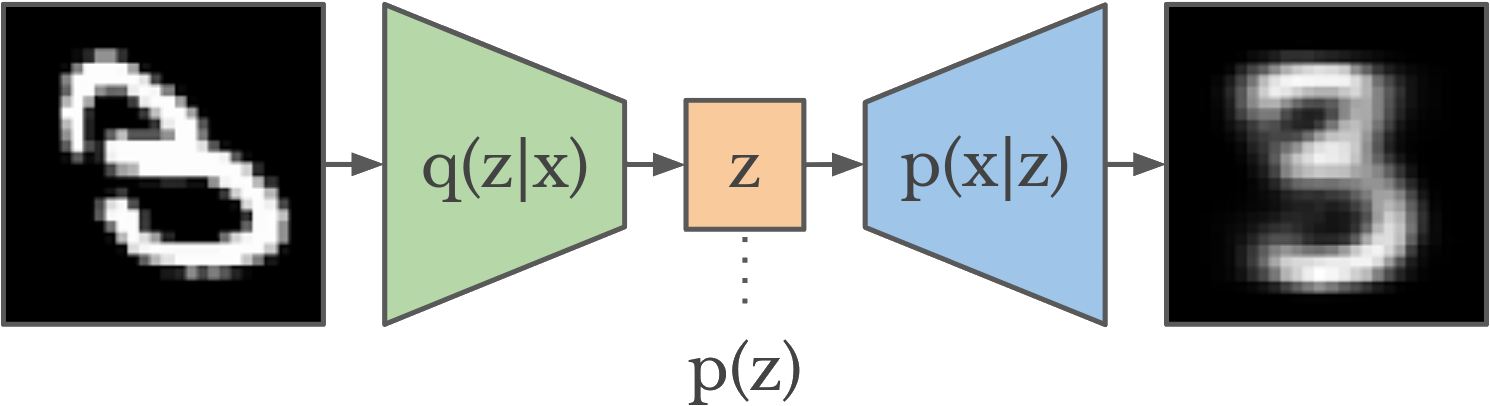
\includegraphics[width=0.8\textwidth]{images/vae.png}
        \caption{VAE Architecture}
        \label{fig:vae}
    \end{figure}
\end{frame}


% Section 3
\section{Score Matching}

\begin{frame}
    \frametitle{Langevin Sampling}
    Score matching provides another approach to generative modelling, inspired by Langevin dynamics.
    \begin{block}{Langevin Sampling}
        \begin{itemize}
            \item Start with a random $x_0$.
            \item Iteratively update it according to
            \[x_{t+1} = x_t + \frac{\epsilon}{2} \nabla_x \log p(x_t) + \epsilon^{1/2} \eta_t\]
            where $\eta_t \sim \mathcal{N}(0, I)$.
        \end{itemize}
    \end{block}
\end{frame}

\begin{frame}
    \frametitle{Score Matching}
    Define the \textbf{score} of $p(x)$ as $\psi(x) = \nabla_x \log p(x)$. Langevin sampling doesn't require knowing $p(x)$ \textit{exactly}, only $\psi(x)$.

    Let's directly model $\psi(x)$ by $\psi_\theta(x)$, our objective being to minimize the expected squared error:
    \[J(\theta) = \mathbb{E}_{p(x)} \left[ \frac{1}{2} \left\| \psi_\theta(x) - \psi(x) \right\|^2 \right]\]

    Under diffrentiability and regularity assumptions,
    \[J(\theta) = \mathbb{E}_{p(x)} \partial \ \psi_\theta(x) + \frac{1}{2} \psi_\theta(x)^2 + C\]
    which can be minimized by gradient descent.
\end{frame}

\begin{frame}
    \frametitle{Annealed Langevin Sampling}
    Langevin sampling doesn't work well on mixed or low-dim data.
    
    \begin{figure}
        \centering
        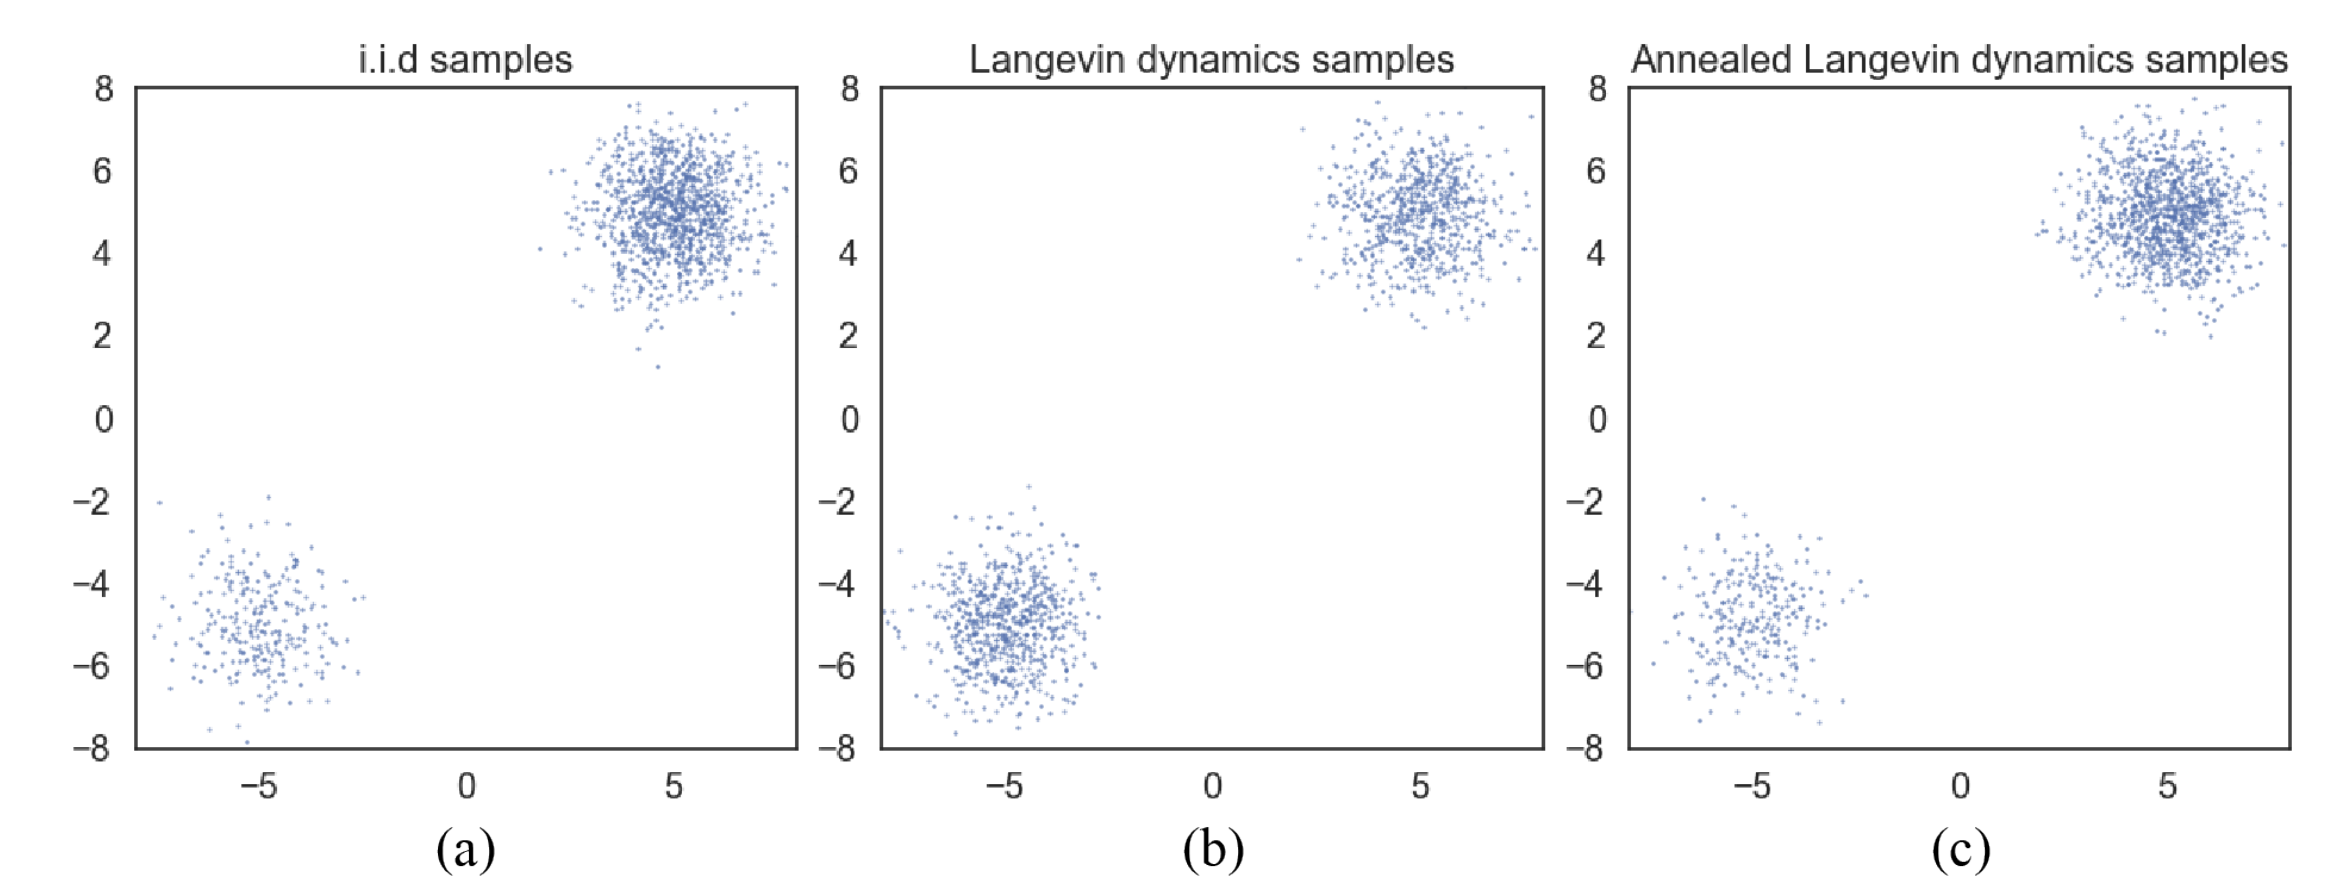
\includegraphics[width=0.8\textwidth]{images/langevin.png}
        \caption[]{Sampling with true scores}
        \label{fig:als}
    \end{figure}

    \begin{block}{Annealed Langevin Sampling (ALS)}
        Model long-range rates of change of $\log p$. Have $\psi(x, \sigma)$ approximate the change in $\log p(x)$ caused by adding $\mathcal{N}(0, \sigma^2)$ noise to $x$.
    \end{block}
\end{frame}

\begin{frame}
    \frametitle{Noise Conditional Score Network}
    Noise Conditional Score Networks (NCSN) optimizes for ALS:
    \begin{figure}
        \centering
        \begin{minipage}{0.45\textwidth}
            \centering
            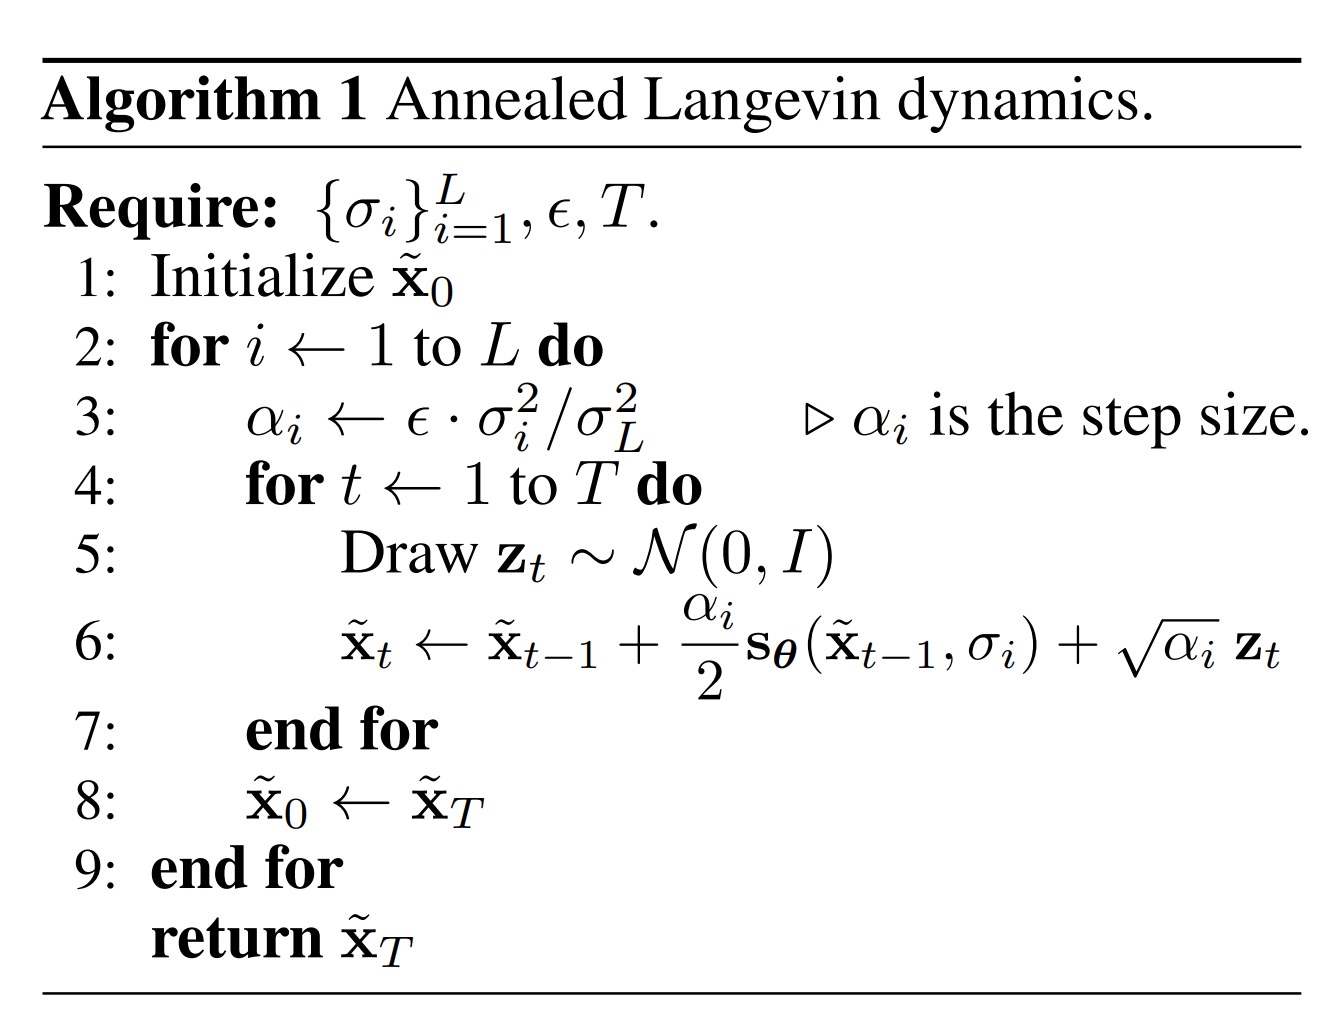
\includegraphics[width=1.2\textwidth]{images/ALD.png}
            % \caption[]{Sampling with true scores}
        \end{minipage}\hfill
        \begin{minipage}{0.45\textwidth}
            \centering
            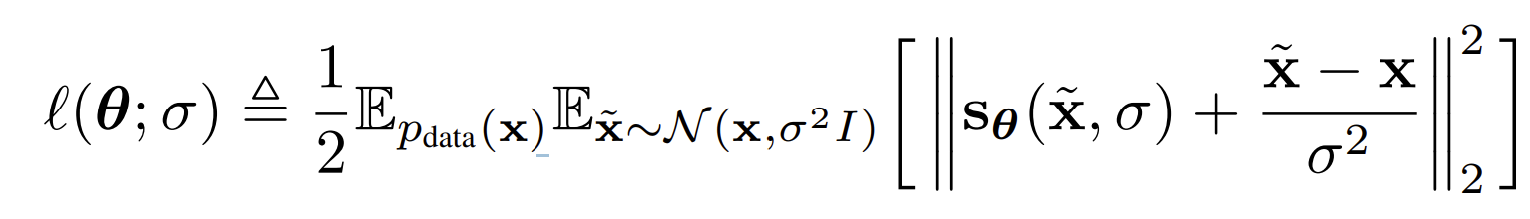
\includegraphics[width=1.1\textwidth]{images/noisy_l.png}
            \\ \\ \\
            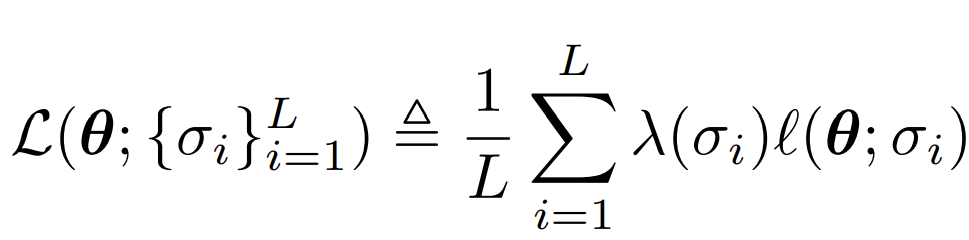
\includegraphics[width=.9\textwidth]{images/noisy_ads_L.png}
        \end{minipage}
    \end{figure}
\end{frame}

\begin{frame}
    \frametitle{Experiments}
    \begin{itemize}
        \item I created synthetic data: 1D mixture of 2 gaussians
        \item I creating 3-layer neural networks (linear + ReLU).
        \item Code at \url{https://github.com/czhang2718/drp-2024}.
    \end{itemize}
    \begin{figure}
        \centering
        \begin{minipage}{0.22\textwidth}
            \centering
            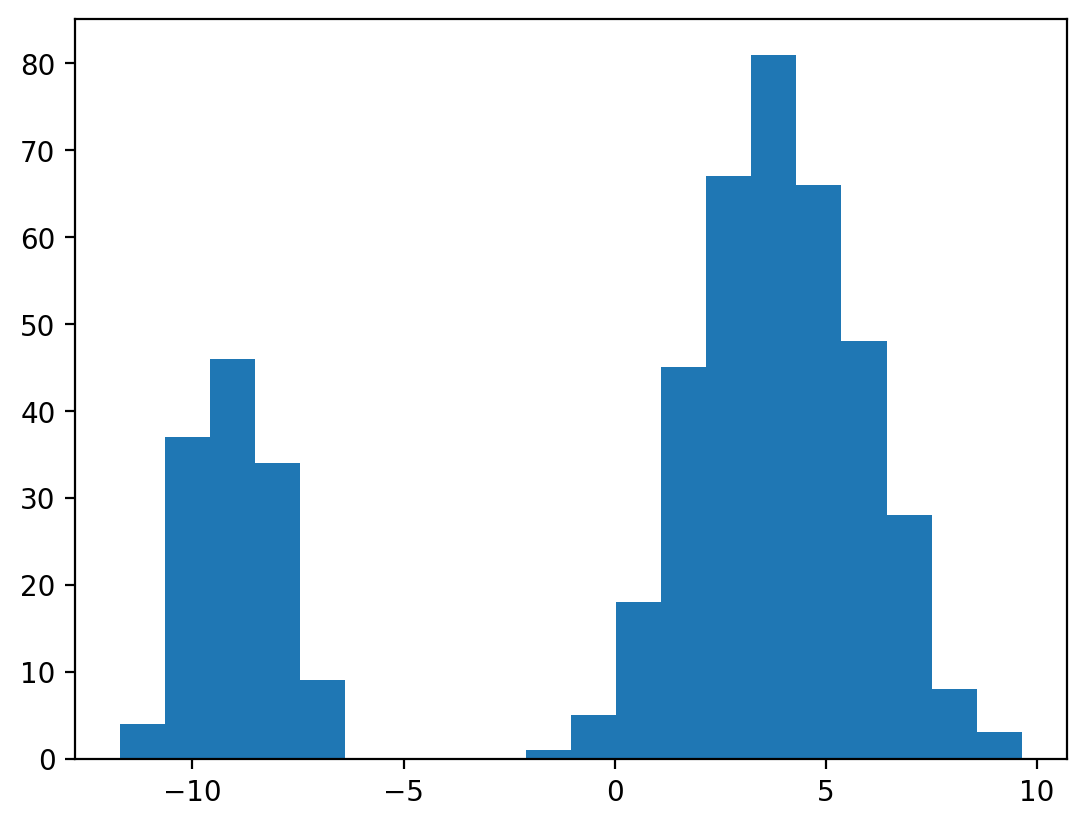
\includegraphics[width=1\textwidth]{images/mix_gauss.png}
            \caption[]{Data}
        \end{minipage}\hfill
        \begin{minipage}{0.22\textwidth}
            \centering
            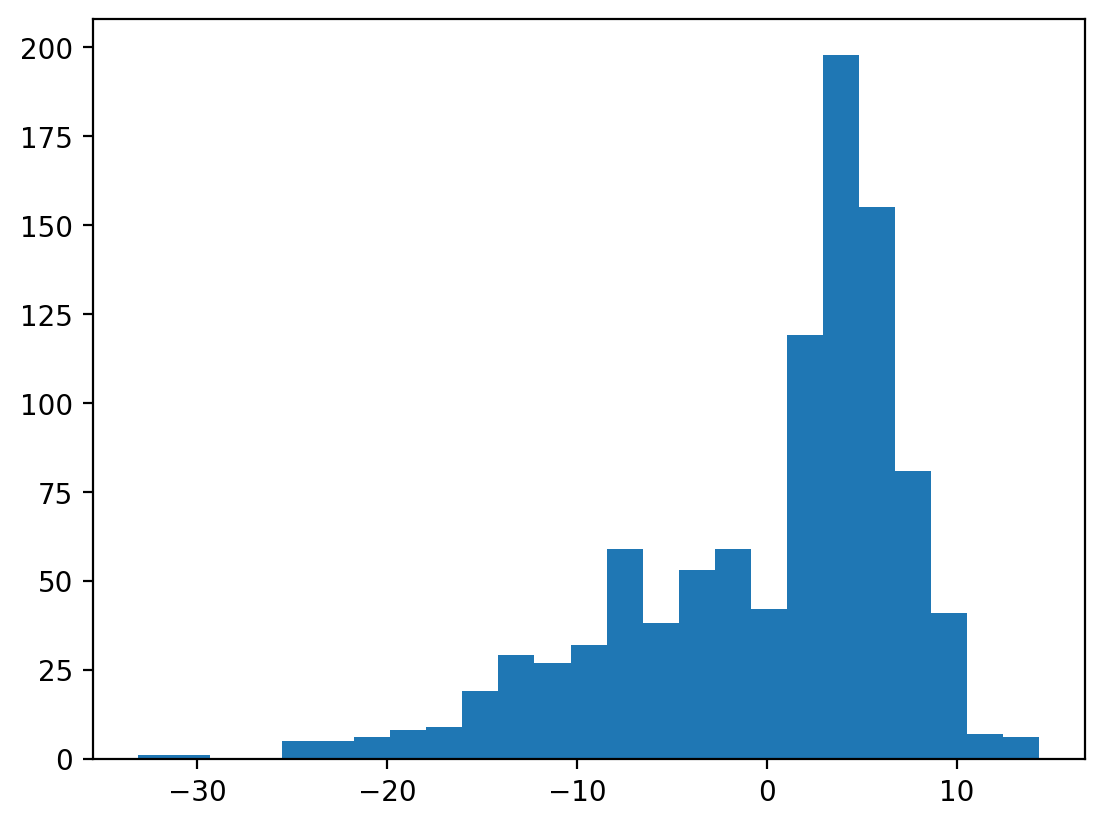
\includegraphics[width=1\textwidth]{images/vae_plot}
            \caption[]{VAE samples}
        \end{minipage}\hfill
        \begin{minipage}{0.22\textwidth}
            \centering
            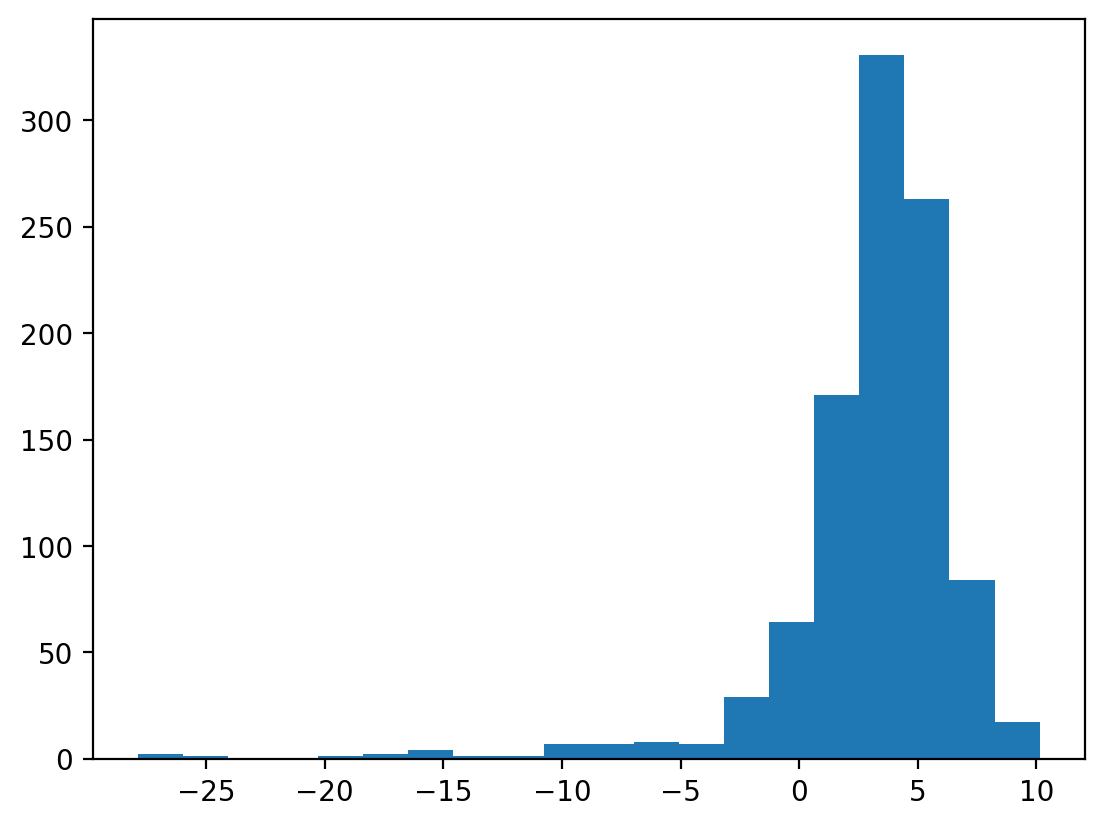
\includegraphics[width=1\textwidth]{images/sm_plot.png}
            \caption[]{SM samples}
        \end{minipage}\hfill
        \begin{minipage}{0.22\textwidth}
            \centering
            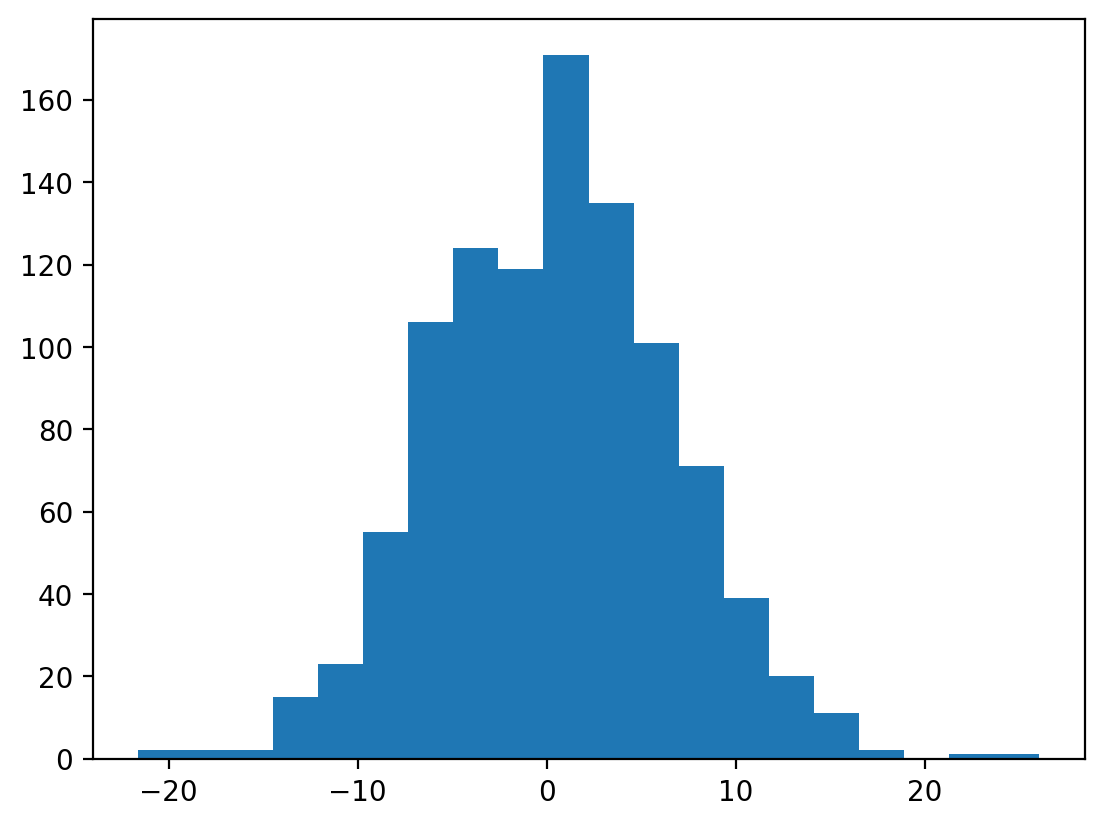
\includegraphics[width=1\textwidth]{images/anneal_sm.png}
            \caption[]{ASM samples}
        \end{minipage}\hfill
    \end{figure}
\end{frame}

% Section 4
\section{Summary}
\begin{frame}
  \frametitle{Summary}
  Variational autoencoders (VAEs) and score matching are two methods for learning a generative model from data.
  
  \begin{block}{VAE}
    Model $x$ using latent variables.
  \end{block}
  \begin{itemize}
    \item Assume prior $z \sim p_\theta(z)$.
    \item Learn an inference model $q_\phi(z|x)$ and generative model $p_\theta(x|z)$.
    \item Sample $\tilde{z} \sim p_\theta(z)$, $\tilde{x} \sim p_\theta(x|\tilde{z})$.
  \end{itemize}
  
  \begin{block}{Score Matching}
    Match first moment $\psi$ of $\log p$.
  \end{block}
  \begin{itemize}
    \item Learn score estimator $\psi(x)$, or $\psi(x, \sigma)$
    \item Sample with (annealed) langevin sampling.
  \end{itemize}
\end{frame}

\begin{frame}
    \frametitle{References}
    \begin{itemize}
        \item Kingma, D. P., \& Welling, M. (2013). Auto-encoding variational bayes. arXiv preprint arXiv:1312.6114.
        \item Hyvärinen, A. (2005). Estimation of non-normalized statistical models by score matching. Journal of Machine Learning Research, 6(Dec), 695-709.
        \item Song, Y. \& Ermon, S. (2019). Generative Modeling by Estimating Gradients of the
        Data Distribution. arXiv preprint arXiv:1907.05600.
    \end{itemize}
\end{frame}

\end{document}
